% Gerado por build_context_results.py; dados de desenvolvimento, não confirmação independente.

\begin{table}[htbp]

\centering\small

\caption{Incremento do contexto adicional em relação ao PSE básico da mesma instância. Variação negativa de custo indica economia; atendimento em pontos percentuais. Nesta rodada, selecionada e protegida coincidem em todas as recomendações.}

\label{tab:contexto_adicional_20261017}

\begin{tabular}{llrr}

\toprule

Base & Instância & $\Delta$ custo (\%) & $\Delta$ atendimento (p.p.) \\

\midrule

Bahia & Classe & -1,176 & -1,265 \\

Bahia & Consequências & +0,000 & +0,000 \\

M5 & Classe & -0,204 & +0,337 \\

M5 & Consequências & -0,035 & -0,003 \\

\bottomrule

\end{tabular}

\end{table}

O módulo adicional foi avaliado reutilizando as matrizes de políticas, sem novos ajustes dos controladores. Foram comparados o PSE básico, todos os atributos admissíveis, a seleção interna de atributos e sua ativação protegida, separadamente nas instâncias por classe e por consequências. Os contrastes usam florestas de 32 árvores com os mesmos parâmetros entre variantes; portanto, suas referências básicas não se confundem com o classificador XGBoost nem com as variantes canônicas de 64 árvores. Não houve atributos adicionais impostos pelo gestor: a variante de atributos fixos coincide com a básica.

Na Bahia, idade, segmento comercial e filial foram incorporados sob a premissa declarada pelo autor de que o cadastro foi extraído diretamente do banco no mesmo período. Essa confirmação não substitui um histórico de alterações por campo. No M5, foram usados departamento do produto, preço histórico, indicação estadual do Supplemental Nutrition Assistance Program (SNAP), programa norte-americano de assistência alimentar, e eventos do último bloco completo de 21 dias do prefixo. Nenhuma informação futura foi usada; o preço funciona como contexto e não altera os custos unitários do ambiente.

A redução de custo por classe na Bahia (1,176\%) veio acompanhada de queda de 1,265 ponto percentual no atendimento. Assim, o ganho de custo não satisfaz isoladamente a finalidade gerencial do AIPE. A instância por consequências manteve exatamente as decisões básicas. No M5, os efeitos selecionados foram pequenos: 0,204\% de economia e 0,337 ponto percentual adicional por classe; por consequências, 0,035\% de economia e variação de -0,003 ponto percentual.

O bootstrap pareado de 5.000 reamostragens por loja/revendedor, preservando produtos e origens no mesmo grupo, produziu para a variação de custo os intervalos condicionais de 95\% [-2,895; 0,371] na Bahia por classe e [-0,684; 0,345] no M5 por classe. Para o atendimento, os respectivos intervalos foram [-2,423; -0,339] e [0,122; 0,609] pontos percentuais. Esses intervalos descrevem os modelos congelados, sem refazer a seleção ou o ajuste; no M5 há somente dez lojas.

Usar todos os atributos também não assegurou vantagem da seleção. No M5 por classe, todos os atributos reduziram o custo em 0,540\%, ante 0,204\% com seleção, mas com menor incremento de atendimento (0,132 ante 0,337 ponto percentual). Na Bahia por classe, todos os atributos elevaram o custo em 0,044\% e reduziram o atendimento. Os contrastes sustentam a necessidade de avaliar informação adicional pelo efeito operacional, sem estabelecer superioridade geral da seleção de atributos ou garantia de atendimento da regra de ativação.

A rodada constitui desenvolvimento: os resultados canônicos já eram conhecidos, as partições de treino dos seletores se sobrepõem e não se realizou confirmação independente. A ampliação permanece opcional; eventuais economias devem ser examinadas com as deteriorações por caso e a relevância definida pelo gestor.

A Figura~\ref{fig:contexto_incremental_20261017} apresenta os contrastes de custo e atendimento e sua incerteza condicional.

\begin{figure}[htbp]

\centering

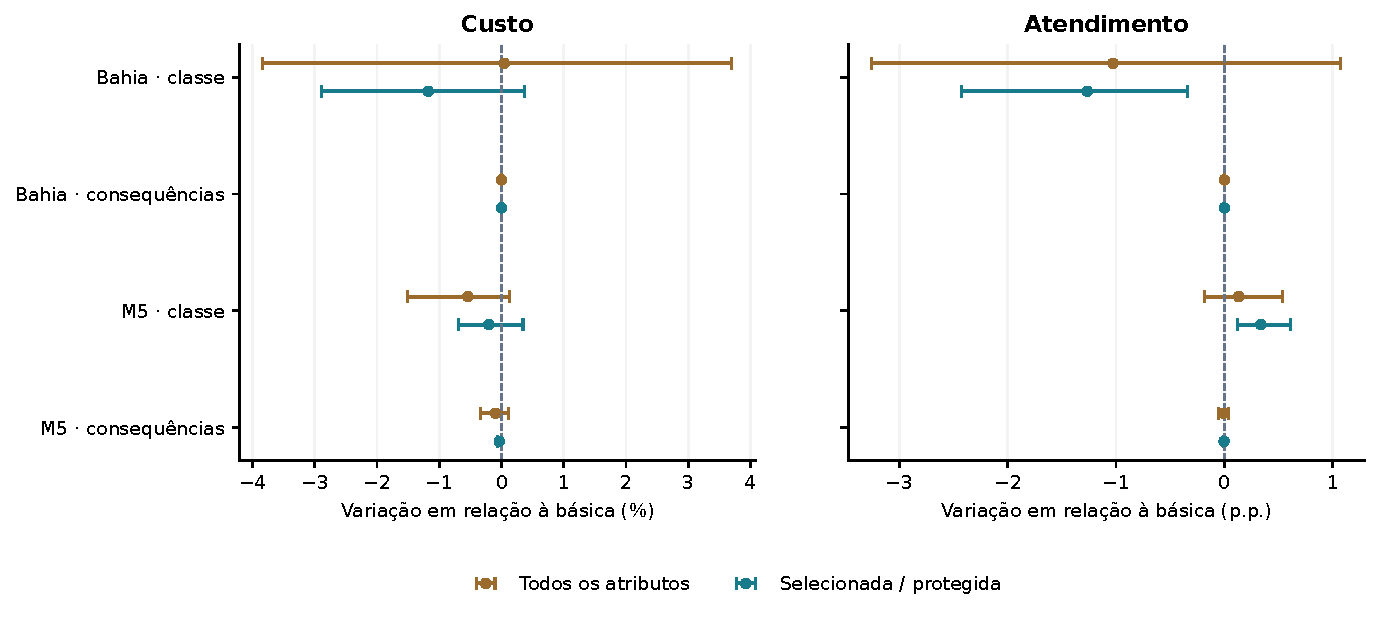
\includegraphics[width=\linewidth]{figures/aipe_contexto_incremental_20261017.pdf}

\caption{Efeito incremental do contexto sobre custo (esquerda) e atendimento (direita), perante o PSE básico da mesma instância. Pontos: variações observadas; barras: intervalos condicionais de 95\% de 5.000 reamostragens pareadas por loja/revendedor, mantendo produtos e origens agrupados. Custo negativo indica economia. Seleção e ativação protegida coincidiram nesta rodada. O bootstrap não refaz os ajustes; o M5 possui dez lojas.}

\label{fig:contexto_incremental_20261017}

\end{figure}
